%    Tercer capítulo: Siintáxis.
%    Ejercicios por Barón L. Miguel.
%    Teoría por Javier Enríquez Mendoza.
%    Empezado el 7/11/22
%    Concluido el 29/11/22

%Gatito Sintáctico
\begin{figure}[htbp]
    \centerline{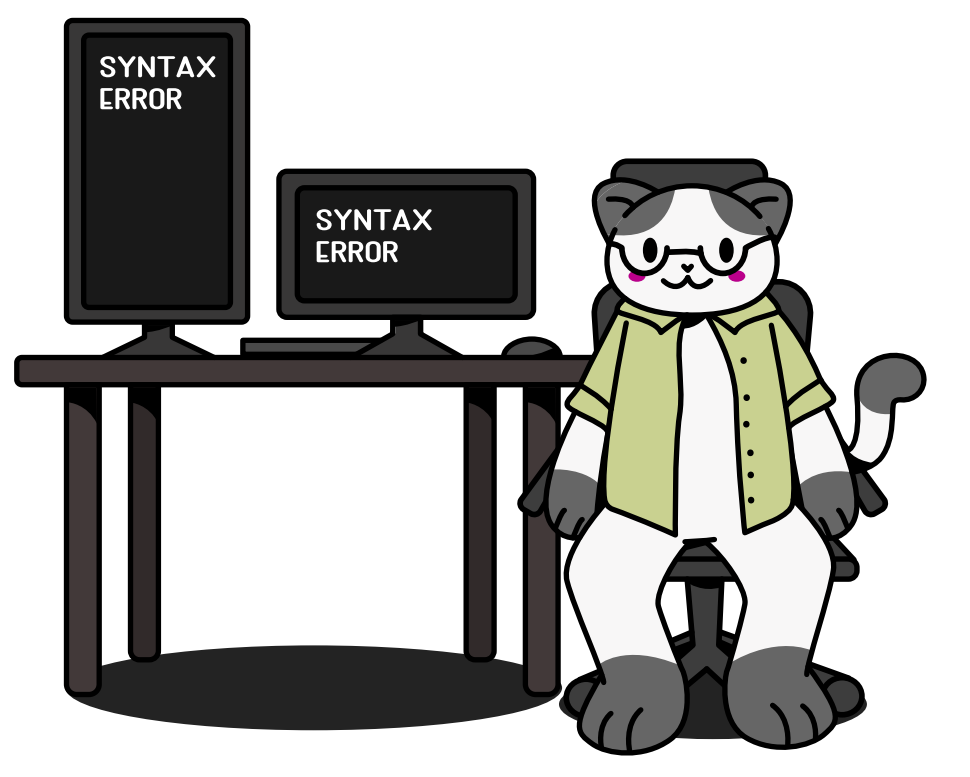
\includegraphics[scale=.38]{assets/03_gatito_sintaxis.PNG}}       
\end{figure}


%Introducción
La sintaxis de un lenguaje de programación permite delimitar el conjunto de las cadenas que pertenecen a este y al mismo tiempo constituye una herramienta de razonamiento para demostrar propiedades utilizando el principio de inducción aplicado a los juicios o reglas que lo definen. \\\\
De forma similar la sintaxis marca la pauta para la definición de funciones como la función de evaluación para obtener el valor asociado a una expresión correctamente construida de un lenguaje de programación y al mismo tiempo será en esta misma estructura donde nos apoyaremos para definir los procesos de análisis para determinar la validez y el tipo de dichas expresiones.\\\\
Para poder comenzar a estudiar los niveles sintácticos de un lenguaje de programación utilizaremos la definición de un nuevo lenguaje el cuál extenderemos con instrucciones a lo largo del desarrollo del manual y lo denominaremos como \textsf{EAB} (expresiones aritmético-booleanas). A partir de la definición de este lenguaje mediante la gramática para generar expresiones y las reglas de inferencia equivalentes abordaremos la construcción y diferencias que existen entre la sintaxis concreta y sintaxis abstracta que se introducen para \textsf{EAB}.\\

\subsection*{Objetivo}
Definir el lenguaje \textsf{EAB} junto con sus diferentes niveles sintácticos, mostrando las principales diferencias que existen entre la sintaxis concreta y abstracta así como estudiar cómo se relacionan proporcionando las reglas para implementar el analizador sintáctico de este mismo.


\subsection*{Planteamiento}
Iniciaremos el estudio de este capítulo brindando las reglas de la sintaxis de \textsf{EAB}\footnote{Este lenguaje es una definición independiente a \textsf{EAL} vista en el \hyperref[sec:intro]{capítulo 1: Introducción}, dado que iremos extendiendo y agregando nuevas instrucciones durante el desarrollo de los siguientes capítulos.} junto con la definición de los nuevos niveles sintácticos; la sintaxis concreta y la sintaxis abstracta, misma que introduce una nueva estructura conocida como árbol de sintaxis abstracta que captura la jerarquía de operación en las instrucciones que se definen en su representación como cadena válida del lenguaje derivada a partir de las reglas definidas en la sintaxis concreta. En particular estudiaremos el proceso mediante el cual una expresión de la sintaxis concreta se relaciona con un árbol de sintaxis abstracta conocido como análisis sintáctico. \\\\
En este nuevo lenguaje vamos a ejemplificar como estos dos niveles sintácticos se relacionan entre sí extendiendo su definición para soportar a los operadores \texttt{if} y \texttt{let}. \\
Posteriormente explicaremos la relación que el operador \texttt{let} introduce con las variables ligadas, variables libres, el alcance de una variable y estudiaremos los conceptos de sustitución y $\alpha$-equivalencia.


%    Section 1: sintaxis concreta y sintaxis abstracta 
\section{Sintaxis concreta}

    La sintaxis concreta se relaciona con la representación gráfica de las cadenas del lenguaje y comúnmente es denotada por una gramática libre de contexto. Esta gramática está pensada para el usuario final, es decir una persona. \\
    A esta capa se le denomina de ''alto nivel'' dado que es un ser humano y no una computadora quien se requiere pueda leer y escribir programas siguiendo las reglas de construcción del lenguaje en cuestión\footnote{Definición formulada a partir de \hyperlink{1}{[1]}, \hyperlink{2}{[2]}, \hyperlink{5}{[5]}, \hyperlink{12}{[12]} y \hyperlink{76}{[76]}}. Vamos a denotar las expresiones del lenguaje con la letra ''\textit{E}''.\\
    Definimos entonces el lenguaje \textsf{EAB}\footnote{Iniciaremos definiendo las instrucciones aritméticas primero y posteriormente agregaremos instrucciones lógico-booleanas con el operador \texttt{if}.} con el siguiente conjunto de juicios: \\
    
    %\begin{definition}
    %    Definición de la grámatica en forma BNF de \textsf{EAB}\footnote{Esta definición fue acuñada a partir de \hyperlink{1}{[1]}, \hyperlink{2}{[2]}, \hyperlink{5}{[5]} y \hyperlink{12}{[12]} adaptada para las instrucciones que nos interesa ejemplificar en este capítulo.}:
    %    \[
    %        \begin{array}{rll}
    %            E & ::= & T \quad |\quad E + T \\
    %            T & ::= & F \quad |\quad T * F \\
    %            F & ::= & N \quad |\quad (E)\\
    %            N & ::= & D \quad |\quad ND \\
    %            D & ::= & 0 \quad |\quad 1 \quad |\quad 2 \quad |\quad 3 \quad |\quad 4 \quad |\quad 5 \quad |\quad 6 \quad |\quad 7 \quad |\quad 8 \quad |\quad 9 
    %        \end{array}
    %    \]
    % \end{definition}

    %De forma equivalente, la gramática previamente mostrada tiene una representación en un conjunto de juicios lógicos.
     
     \begin{definition}
        Sintaxis concreta en forma de juicios lógicos para cada regla en nuestra gramática para \textsf{EAB}\footnote{Esta definición fue acuñada a partir de \hyperlink{1}{[1]}, \hyperlink{2}{[2]}, \hyperlink{5}{[5]} y \hyperlink{12}{[12]} adaptada para las instrucciones que nos interesa ejemplificar en este capítulo.}: 
        \[
            \begin{array}{cccc}
            \inference{}{0\;{\text{D}}}&
            \inference{}{1\;{\text{D}}}&
            \cdots&
            \inference{}{9\;{\text{D}}}
            \end{array}
        \]
        \[
            \begin{array}{cc}
            \inference{d\;{\sf \text{D}}}{d\;{\text{N}}}&
            \inference{n\;{\sf \text{N}}&d\;{\text{D}}}{nd\;{\text{N}}}\\
            &\\
            \inference{n\;{\sf \text{N}}}{n\;{\sf \text{F}}}&
            \inference{e\;{\sf \text{E}}}{(e)\;{\sf \text{F}}}\\
            &\\
            \inference{f\;{\sf \text{F}}}{\text{F}\;{\sf \text{T}}}&
            \inference{t\;{\sf \text{T}}&f\;{\sf \text{F}}}{t*f\;{\sf \text{T}}}\\
            &\\
            \inference{t\;{\sf \text{T}}}{t\;{\sf \text{E}}}&
            \inference{e\;{\sf \text{E}}&t\;{\sf \text{T}}}{e+t\quad{\sf \text{E}}}
            \end{array}
        \]
    \end{definition}

    \section{Sintaxis abstracta}

    La sintaxis abstracta por otra parte como su nombre lo indica se relaciona con la abstracción de la estructura del lenguaje y comúnmente es definida mediante reglas de inferencia para construir un árbol sintáctico donde cada nodo corresponde a una instrucción o operador
     y los hijos a los parámetros que recibe dicha instrucción\footnote{Definición formulada a partir de \hyperlink{5}{[5]}, \hyperlink{12}{[12]}, \hyperlink{77}{[77]}, \hyperlink{78}{[78]} y \hyperlink{79}{[79]}.}. \\\\
    Las hojas de los árboles sintácticos corresponden a los tipos primitivos del lenguaje (enteros, booleanos, caracteres, etc.). En este capítulo vamos a denotar a un árbol de sintaxis abstracta como ''\textit{ASA}''.\\\\
    Los árboles sintácticos son útiles para definir la jerarquía de las operaciones a realizar durante la evaluación de una expresión bien formada de un lenguaje y eliminar la ambigüedad del mismo dado que un árbol de sintaxis abstracta es único sin importar la representación que una expresión tenga en sintaxis concreta. \\\\ 
    %Como mencionamos, existe una representación en sintaxis abstracta para cada expresión bien formada de nuestro lenguaje \textsf{EAB}. Vamos a denotar como ''\textit{ASA}'' a dicha estructura, la cual está definida por el siguiente conjunto de reglas que nos permiten construir el árbol sintáctico correspondiente a dicha expresión. \\

    \begin{definition}
        Sintaxis abstracta de \textsf{EAB}\footnote{Esta definición fue acuñada a partir de \hyperlink{1}{[1]}, \hyperlink{2}{[2]}, \hyperlink{5}{[5]} y \hyperlink{12}{[12]} adaptada para las instrucciones que nos interesa ejemplificar en este capítulo.}
        \[
            \begin{array}{ccc}
                \inference{n\in\N}{num[n]\;\text{ASA}}&
                \inference{t_1\;\textit{ASA}&t_2\;\textit{ASA}}{sum(t_1,t_2)\;\textit{ASA}}&
                \inference{t_1\;\textit{ASA}&t_2\;\textit{ASA}}{prod(t_1,t_2)\;\textit{ASA}}
            \end{array}
        \]
        En donde el predicado $t_1\ ASA$ se lee como: '' $t_1$ es un árbol de sintaxis abstracta''.\\\\
        Es importante notar que los árboles de sintaxis abstracta aunque similares a la expresión en sintaxis concreta que representan corresponden a una categoría distinta de los niveles sintácticos para \textsf{EAB}.
        
    \end{definition}

   \subsection{Analizador sintáctico}
    Al proceso mediante el cual se obtiene el árbol de sintaxis abstracta de una expresión en sintaxis concreta se le conoce como análisis sintáctico. Es importante notar que no siempre será posible encontrar el árbol de sintaxis abstracta (por ejemplo si la expresión que analizamos no es derivable de las reglas de la sintaxis concreta).\\\\
    De tal forma que el objetivo ahora será definir formalmente la relación entre ambos niveles donde el siguiente juicio es válido:\footnote{La definición de esta relación fue formulada a partir de \hyperlink{1}{[1]}, \hyperlink{5}{[5]} y \hyperlink{12}{[12]}, se refiere a las siguientes publicaciones para un estudio en profundidad sobre los niveles sintácticos de los lenguajes de programación: \hyperlink{76}{[76]}, \hyperlink{77}{[77]}, \hyperlink{78}{[78]} y \hyperlink{79}{[79]}}
            \[ e\  E \longleftrightarrow a\ ASA \]
    Esta relación se interpreta como ''a es el árbol de sintaxis abstracta asociado a la expresión e''. Definimos entonces las reglas para implementarla en \textsf{EAB} como sigue:

    \bigskip

    \begin{definition}
        Analizador síntactico para expresiones de lenguaje de EAB\footnote{Definición formulada a partir de \hyperlink{1}{[1]}, \hyperlink{2}{[2]}, \hyperlink{5}{[5]} y \hyperlink{12}{[12]}}
        \[
            \begin{array}{ccc}
                \inference{e\;{\sf N}&e\in\N}{e\;{\sf F}\longleftrightarrow num[e]\;\textit{ASA}}[\textit{(num)}]&
                \quad&
                \inference{e\;{\sf E}\longleftrightarrow a\;\textit{ASA}}{(e)\;{\sf F}\longleftrightarrow a\;\textit{ASA}}[\textit{(parentE)}]\\
                &&\\
                \inference{e\;{\sf F}\longleftrightarrow a\;\textit{ASA}}{e\;{\sf T}\longleftrightarrow a\;\textit{ASA}}[\textit{(fact)}]&
                \quad&
                \inference{e_1\;{\sf T}\longleftrightarrow a_1\;\textit{ASA}&e_2\;{\sf F}\longleftrightarrow a_2\;\textit{ASA}}{e_1*e_2\;{\sf T}\longleftrightarrow prod(a_1,a_2)\;\textit{ASA}}[\textit{(prod)}]\\
                &&\\
                \inference{e\;{\sf T}\longleftrightarrow a\;\textit{ASA}}{e\;{\sf E}\longleftrightarrow a\;\textit{ASA}}[\textit{(exprE)}]&
                \quad&
                \inference{e_1\;{\sf E}\longleftrightarrow a_1\;\textit{ASA}&e_2\;{\sf T}\longleftrightarrow a_2\;\textit{ASA}}{e_1+e_2\;{\sf T}\longleftrightarrow sum(a_1,a_2)\;\textit{ASA}}[\textit{(sum)}]
            \end{array}
        \]
    \end{definition}

    \bigskip
    
    Ahora queremos extender EAB agregando instrucciones booleanas que permitan tener condicionales en nuestras expresiones de lenguaje. Es decir queremos agregar las constantes booleanas \texttt{True} y \texttt{False}, el operador \texttt{if} ... \texttt{then} simple y el operador \texttt{if}... \texttt{then} ... \texttt{else} ... así como parentizado de expresiones para evitar condiciones de ''else colgante''\footnote{Éste problema es conocido en inglés como ''$dangling\ else$'' recurrente en la implementación de \textit{parsers} en el que una cláusula else opcional en una declaración if-then(-else) da como resultado que los condicionales anidados sean ambiguos. \hyperlink{90}{[90]}} y ambigüedad (esta regla puede ser modelada encerrando entre paréntesis la expresión inmediata a evaluar en la instrucción \texttt{then}).

    \bigskip
    
    \begin{exercise}        
        Define la sintaxis concreta para extender nuestro lenguaje \textsf{EAB} con las instrucciones lógicas previamente discutidas\footnote{Definición formulada a partir de \hyperlink{1}{[1]}, \hyperlink{5}{[5]}, \hyperlink{8}{[8]} y \hyperlink{12}{[12]} }
        \[ 
            \inference{}{\texttt{True} \text{ B}} \quad \inference{}{\texttt{False} \text{ B}}
        \]
        \[ 
             \inference{c \text{ B } t \text{ LE }  c \text{ E}}{\texttt{if $c$ then $t$ else $e$ $E$}} \inference{c \text{ B } t \text{ LE}}{\texttt{if $c$ then $t$ E}} \inference{x \text{ B }}{x \text{ LE}}
        \]
        \[
            \inference{e \text{ E}}{(e) \text{ LE}} \inference{e \text{ LE}}{ e \text{ E}}
        \]
    \end{exercise}

    \bigskip

%  Definición alternativa
%        \[ 
%            \inference{\x \in \{a,b\} }{\text{ x Input}}
%            \inference{\x \in \{\top,\bot\} }{\text{ x Output}}
%        \]
%        \[
%            \inference{c \text{ Input } t \text{ ASA  } e \text{ ASA}}{ \textbf{if(} \text{c t e} \textbf{)} \text{ ASA}} 
%            \inference{x \text{ Output }}{ \text{(Out x)} \text{ ASA}}
%        \]
    
    \begin{exercise}
        Define los juicios que componen la sintaxis abstracta para el operador \texttt{If}\footnote{Definición formulada a partir de \hyperlink{1}{[1]}, \hyperlink{5}{[5]}, \hyperlink{8}{[8]} y \hyperlink{12}{[12]} }\\
        \[
            \inference{\texttt{True} \text{ B} }{\textit{T} \textit{ ASA}}
            \inference{\texttt{False} \text{ B} }{\textit{F} \textit{ ASA}}
        \]
        \[
            \inference{c \textit{ ASA } t \textit{ ASA  } e \textit{ ASA}}{ \textit{if} \text{(} \textit{c t e} \text{)} \textit{ ASA}} 
            \inference{c \textit{ ASA } t \text{ ASA  }}{ \textit{if(} \textit{c t} \text{)} \textit{ ASA}} 
        \]
    \end{exercise}

    \bigskip
    
    \begin{exercise}
        Define las reglas del analizador sintáctico para el operador \texttt{If}\footnote{Definición formulada a partir de \hyperlink{1}{[1]}, \hyperlink{5}{[5]}, \hyperlink{8}{[8]} y \hyperlink{12}{[12]} }.
        \[
            \inference{}{\texttt{True} \text{ B} \longleftrightarrow \text{T} \textit{ ASA}}[\textit{(true)}] 
            \inference{}{\texttt{False} \text{ B} \longleftrightarrow \text{F} \textit{ ASA}}[\textit{(false)}]
        \]
        \[
            \inference{\text{$c$ B} \longleftrightarrow \textit{c'}  \textit{ ASA } \quad \text{$t$ LE } \longleftrightarrow \text{$t'$ ASA } \quad \text{$e$ E } \longleftrightarrow \text{e'} \textit{ ASA }}{\texttt{if $c$ then $t$ else $e$ E } \longleftrightarrow \textit{if(c' t' e')} \textit{ ASA} }[$(if_e)$]
        \]
        \[
            \inference{\text{$c$ B} \longleftrightarrow \textit{c'} \textit{ ASA} \quad \text{ $t$ LE} \longleftrightarrow \textit{t' ASA } }
            { \texttt{if($c$ then $t$) E} \longleftrightarrow  \textit{if(c' t')} \textit{ ASA} }[$(if_s)$]
        \]
        \[
            \inference{ \text{$c$ E} \longleftrightarrow \textit{e'} \textit{ ASA}}{\text{($e$) LE} \longleftrightarrow \textit{e'} \textit{ ASA}}[\textit{(parentB)}] \;
            \inference{\text{$c$ B} \longleftrightarrow \textit{c'} \textit{ ASA}}{\text{$c$ LE} \longleftrightarrow \textit{c'} \textit{ ASA}}[\textit{(bool)}] \;
            \inference{\text{$e$ LE} \longleftrightarrow \textit{e'} \textit{ ASA}}{\text{$e$ E} \longleftrightarrow \textit{e'} \textit{ ASA}}[\textit{(exprB)}]
        \]
    \end{exercise}


\section{El operador let}

    Ahora necesitamos extender aún mas \textsf{EAB} para incluir expresiones de tipo: 
    \[\texttt{let } \textit{ x } \text{=} \textit{ $e_1$ } \texttt{in} \textit{ $e_2$ }  \texttt{end}\]

    Donde las apariciones de la variable \textit{x} serán sustituidas por $e_1$ en $e_2$.
    
    Para este propósito se tiene que definir la sintaxis del operador \texttt{let} y el concepto de ligado de variables. \\

    \begin{exercise}
        Proporciona las sintaxis concreta para agregar las instrucciones \texttt{let} de tal forma que sea congruente con las especificación mencionada anteriormente\footnote{Definición formulada a partir de \hyperlink{1}{[1]}, \hyperlink{5}{[5]}, \hyperlink{12}{[12]} y \hyperlink{81}{[81]} }.

        \[
            \inference{e \text{ identificador}}{e\text{ V}}[\textit{(var) }]
            \inference{e\text{ V}}{e\text{ B}}[\textit{(vIn) }]
            \inference{e\text{ V}}{e\text{ F}}[\textit{(vfac) }]
            \inference{x\text{ V} \quad \text{$e_1$ E} \quad \text{$e_2$ E}}{ \texttt{let $x$ = $e_1$ in $e_2$ end E}}[\textit{(let)}]
        \]
    \end{exercise}


    La sintaxis abstracta de orden superior define un tratamiento especial para las variables que se introducen con el operador \texttt{let} así como el alcance y ligado de las mismas. Esta sintaxis abstrae estos niveles como parte del metalenguaje con el que se define el árbol de sintaxis abstracta, es decir vamos a delimitar el rango de aplicación de la variable con el árbol que definiremos para el operador mismo.\\\\
    Extenderemos nuestro lenguaje \textsf{EAB} agregando el árbol de sintaxis abstracta \textit{x.t} que indica que la variable \textit{x} está ligada
    en el árbol \textit{t}, a este \textit{ASA} se le llama abstracción\footnote{Definición acuñada a partir de \hyperlink{1}{[1]}, \hyperlink{2}{[2]}, \hyperlink{5}{[5]}, \hyperlink{12}{[12]}, \hyperlink{80}{[80]} y \hyperlink{81}{[81]}}. Esto es importante dado que al introducir las variables ligadas y su alcance tenemos que delimitar la expresión en la que la sustitución ocurrirá.

    \begin{exercise}
        Proporciona las sintaxis Abstracta para agregar las instrucción \texttt{let}\footnote{Definición formulada a partir de \hyperlink{1}{[1]}, \hyperlink{5}{[5]}, \hyperlink{12}{[12]} y \hyperlink{81}{[81]} } considerando el \textit{ASA} \textit{x.t}.
        \[
            \inference{\text{$x$ identificador}}{\text{var[$x$] \textit{ASA}}}[] 
            \inference{\textit{$a_1$ \textit{ASA}} \quad \textit{$a_2$ \textit{ASA}} }{\text{\textit{let(}$a_1$, $x$.$a_2$\textit{)} \textit{ASA}}}[]
        \]
    \end{exercise}

    \bigskip

    \begin{exercise}
         Define las reglas del analizador sintáctico para agregar las instrucción \texttt{let}\footnote{Definición formulada a partir de \hyperlink{1}{[1]}, \hyperlink{5}{[5]}, \hyperlink{12}{[12]} y \hyperlink{81}{[81]} }.
         \[
            \inference{x \text{ identificador}}{\text{$x$ V} \longleftrightarrow \text{var[$x$] \textit{ASA}}}[\textit{ vara }]
            \inference{\text{$x$ V} \quad \text{$e_1$ E} \longleftrightarrow \textit{$a_1$ ASA} \quad \text{$e_2$ E} \longleftrightarrow \text{$a_2$ \textit{ASA}} }
                      {\texttt{let $x$ = $e_1$ in $e_2$ end E} \longleftrightarrow \textit{let($a_1$ $x$.$a_2$) \textit{ASA}}}[\textit{leta}]
         \]
    \end{exercise}

    \bigskip

    A continuación tenemos tres ejemplos que nos van a ayudar a ilustrar la aplicación de las reglas que hemos definido hasta el momento para construir los \textit{ASA} de \textsf{EAB} partiendo de expresiones derivadas de las reglas de la sintaxis concreta.

    \bigskip

    \begin{exercise}
        Obtén la representación en sintaxis abstracta partiendo de la sintaxis concreta de las siguiente expresión: \\\\
        \texttt{let} $x$ = 1 \texttt{in} $x$ + 1 \texttt{end}\\
        \[
            \textit{let(num[1], $x.$var[$x$]+1)}\ ASA
        \]
    \end{exercise}

    \begin{exercise}
        Obtén la representación en sintaxis abstracta partiendo de la sintaxis concreta de las siguiente expresión: \\\\
        \texttt{let} $y$ = \texttt{if} \texttt{True} \texttt{then} 1 \texttt{else} 0 \texttt{in} \texttt{if} $x$ \texttt{then} \texttt{False} \texttt{end}\\
        \[
            \textit{let(if(T, num[1], num[0]), $y$.if(var[$x$], F))\ ASA}
        \]
    \end{exercise}

    \begin{exercise}
        Obtén la representación en sintaxis abstracta partiendo de la sintaxis concreta de las siguiente expresión: \\
        
        \texttt{let $x$ = False} \texttt{in} \texttt{if} $x$ \texttt{then} (\texttt{if} $\alpha$ \texttt{then} (\texttt{if} $\alpha$ \texttt{then} 4)) \texttt{else False} \texttt{end}\\
        \[
            \textit{let(F, x.if(var[x], if(var[$\alpha$], if(var[$\alpha$], num[4])), F)) ASA}
        \]        
    \end{exercise}

    \bigskip

    \subsection{Clasificación de variables en el operador let}
    
    La introducción de nuestro nuevo operador \texttt{let} acarrea consigo la definición de ligado de una variable, variable ligada\footnote{Aún que los nombres son similares ligado de una variable y variable ligada corresponden a dos definiciones distintas.}, variable libre y la definición de la función de sustitución junto con la función para obtener variables libres de una expresión, mismas que serán mostradas a continuación y serán de utilidad para resolver el resto de los ejercicios presentes en este capítulo.\\
    
    \begin{definition}Ligado de una variable: la instancia de ligado de una variable es aquella que da a esta su valor\footnote{Definición formulada de \hyperlink{2}{[2]}, \hyperlink{5}{[5]}, \hyperlink{12}{[12]}, \hyperlink{80}{[80]} y \hyperlink{81}{[81]}}. Es decir, es la aparición de la variable en donde esta es definida. \\\\
    De tal forma que si tenemos la siguiente expresión: \[ \texttt{let } x = e_1 \texttt{ in } e_2 \texttt{ end } \] Decimos que $x = e_1$ es el ligado de la variable \textit{x} en la instrucción \texttt{let}.
    \end{definition}

    \bigskip

    \begin{definition}Variable ligada: sea \textit{x.t} un \textit{ASA}, decimos que \textit{x} está ligada en \textit{t} para todas las apariciones de \textit{x}\footnote{Definición formulada de \hyperlink{2}{[2]}, \hyperlink{5}{[5]}, \hyperlink{12}{[12]}, \hyperlink{80}{[80]} y \hyperlink{81}{[81]}}.\\\\
    De tal forma que si tenemos la siguiente expresión: \[ \texttt{let } x = e_1 \texttt{ in } e_2 \texttt{ end } \] Decimos que $x $ es la variable ligada en $e_2$ dentro de nuestra expresión \texttt{let}.
    \end{definition}

    \bigskip

    \begin{definition}Variable libre: una variable está libre en una expresión, si no se encuentra dentro del alcance de una variable de ligado con su nombre. Es decir, una variable es libre si no está ligada\footnote{Definición formulada de  \hyperlink{2}{[2]}, \hyperlink{5}{[5]}, \hyperlink{12}{[12]}, \hyperlink{80}{[80]} y \hyperlink{81}{[81]}}.\\\\
    De tal forma que si tenemos la siguiente expresión: \[ \texttt{let } x = e_1 \texttt{ in } y \texttt{ end } \] Decimos que $y$ es una variable libre en nuestra expresión \texttt{let}.
    \end{definition}

    \bigskip
    
    \begin{definition}Función para obtener las variables libres de una expresión: dado el árbol de sintaxis abstracta $a$  definimos el conjunto de variables libres de la expresión\footnote{Definición extraída de  \hyperlink{2}{[2]}, \hyperlink{5}{[5]}, \hyperlink{12}{[12]}, \hyperlink{80}{[80]} y \hyperlink{81}{[81]}}, denotado $FV(a)$ como sigue:
        \[
            \begin{array}{lcl}
                FV(x)&=&\{x\}\\
                FV(O(a_1,\cdots,a_n))&=&FV(a_1)\cup\cdots\cup FV(a_n)\\
                FV(x.a)&=&FV(a)\backslash\{x\}
            \end{array}
        \]
    \end{definition}

    \bigskip

    \begin{exercise}
    Dada la siguiente expresión \texttt{let} definida como:
    \begin{align*}
    	e=_{\text{def}}\texttt{let  }
    		x&= \texttt{let }x = (2 + 4) \texttt{ in } x+1 \texttt{ end }
    		\texttt{ in }\\
    		 &\texttt{let }y=(x \ast 2)+x 
    		 	\texttt{ in } \\
    		 & \qquad(x\ast y) + \texttt{let }z=7 \texttt{ in } 
    		 						y+z 
    		 				\texttt{ end }\\
    		 &\texttt{ end }\\
    	\texttt{ end }&
    \end{align*}

    Por cada subexpresión \textsf{let} en $e$ (inclusive) proporciona el alcance indicado o subrayando las variables ligadas.

    
    \begin{align*}
    	e=_{\text{def}}\texttt{let  }
    		\setulcolor{blue}\textit{\ul{x}}&= \texttt{let }\setulcolor{purple}\textit{\ul{x}} = (2 + 4) \texttt{ in } \setulcolor{purple}\textit{\ul{x}}+1 \texttt{ end }
    		\texttt{ in }\\
    		 &\texttt{let }\setulcolor{green}\textit{\ul{y}} =( \setulcolor{blue}\textit{\ul{x}} \ast 2)+ \setulcolor{blue}\textit{\ul{x}} 
    		 	\texttt{ in } \\
    		 & \qquad( \setulcolor{blue}\textit{\ul{x}}\ast \setulcolor{green}\textit{\ul{y}}) + \texttt{let }\setulcolor{orange}\textit{\ul{z}}=7 \texttt{ in } 
    		 						\setulcolor{green}\textit{\ul{y}}+\setulcolor{orange}\textit{\ul{z}}
    		 				\texttt{ end }\\
    		 &\texttt{ end }\\
    	\texttt{ end }&
    \end{align*}
    
    \end{exercise}

    \bigskip

    \begin{exercise}
    Escribe cada subexpresión let en $e$ (inclusive) indicando la variable de ligado y la expresión \texttt{let} para la cual la variable de ligado tiene alcance.
    
        \begin{align*}
    	\texttt{let  }
    		\setulcolor{blue}\textit{\ul{x}}&= \texttt{let }x = (2 + 4) \texttt{ in } x+1 \texttt{ end }
    		\texttt{ in }\\
    		 &\texttt{let }y=(x \ast 2)+x 
    		 	\texttt{ in } \\
    		 & \qquad(x\ast y) + \texttt{let }z=7 \texttt{ in } 
    		 						y+z 
    		 				\texttt{ end }\\
    		 &\texttt{ end }\\
    	\texttt{ end }&
        \end{align*}

        La siguiente expresión \texttt{let} es la que le da su valor a la variable más externa definida en $e$ la cual se identifica como: 
        \begin{align*}
    		\texttt{let }\setulcolor{purple}\texttt{\ul{x}} = (2 + 4) \texttt{ in } x+1 \texttt{ end }
        \end{align*}

        La expresión \texttt{let} que continua está delimitada por los marcadores más externos \texttt{in} \texttt{end} en $e$ y se identifica como: 
        \begin{align*}
    	   &\texttt{let }\setulcolor{green}\texttt{\ul{y}}=(x \ast 2)+x  \texttt{ in } \\	 
                        &\qquad(x\ast y) + \texttt{let }z=7 \texttt{ in } y+z \texttt{ end }\\
    		 &\texttt{ end }\\
        \end{align*}

        La útltima expresión \texttt{let} está delimitada por los marcadores \texttt{in} \texttt{end} de la expresión anterior y se identifica como: 
        \begin{align*}
                 &\texttt{let } \setulcolor{orange}\texttt{\ul{z}}=7 \texttt{ in } y+z \texttt{ end }\\
        \end{align*}
    \end{exercise}

    \bigskip

    \begin{exercise}
        La expresión $e$ se puede evaluar a un valor? si sí muestra el procedimiento para la evaluación informal (aún no definimos la manera en la que se va a evaluar la expresiones del lenguaje \textsf{EAB} pero se puede dar una idea de la evaluación partiendo de la descripción hecha en el capítulo).
    
        \begin{align*}
        	e=_{\text{def}}\texttt{let  }
        		x&= \texttt{let }x = (2 + 4) \texttt{ in } x+1 \texttt{ end }
        		\texttt{ in }\\
        		 &\texttt{let }y=(x \ast 2)+x 
        		 	\texttt{ in } \\
        		 & \qquad(x\ast y) + \texttt{let }z=7 \texttt{ in } 
        		 						y+z 
        		 				\texttt{ end }\\
        		 &\texttt{ end }\\
        	\texttt{ end }&
        \end{align*}
    
        Primero se resuelve la expresión let que la da valor a la variable $x$ en la expresión $e$:
        \[
            \texttt{let }x = (2 + 4) \texttt{ in } x+1 \texttt{ end } 
             = (2+4) + 1 
             = (6) + 1
             = 7
        \]
        Se sustituye este valor en el cuerpo de $e$ resultando en la siguiente expresión:
        \begin{align*}
            &\texttt{let }y =(7 \ast 2)+7  \texttt{ in }\newline
            &\qquad(7\ast y) + \texttt{let }z=7 \texttt{ in } y+z \texttt{ end }\newline
            &\texttt{ end }
        \end{align*}
        Resolviendo la operación para dar variable a la variable y obtenemos el siguiente resultado: 
        \[
            y = (7 \ast 2) + 7 
            = (14) + 7 
            = 21
        \]
        Sustituyendo el nuevo valor en el cuerpo de la expresión anterior se obtiene:
        \begin{align*}
                 & = (7 \ast 21) + \texttt{let } z=7 \texttt{ in } 21 + z \texttt{ end }
        \end{align*}
        Resolviendo las operaciones y la sustitución de la variable $z$ en el cuerpo de la expresión let se obtiene:
        \[
            = 147 + 21 + 7
            = 168 + 7
            = 175
        \]

    \end{exercise}

    \bigskip
    
    \begin{exercise}
        En nuestra expresión $e$ hay variables libres, argumenta por qué si o por qué no. \\
    
        No, todas las variables definidas en la expresión $e$ están asociadas a un operador \texttt{let} marcando su alcance en las expresiones anidadas presentes por lo que ninguna variable aparece sin su respectiva asociación.
    \end{exercise}


\section{Sustitución y $\alpha$-equivalencias}
    Para finalizar este capítulo se introduce el concepto de alfa equivalencia:

    \begin{definition}$\alpha$-equivalencia: se dice que dos expresiones $e_1$ y $e_2$ son $\alpha$-equivalentes si y sólo si difieren únicamente en el nombre de las variables ligadas\footnote{La notación de la relación de $\alpha$-equivalencia fue extraída de \hyperlink{1}{[1]}, \hyperlink{5}{[5]} y \hyperlink{12}{[12]}, la definición formulada a partir de \hyperlink{81}{[81]} y \hyperlink{89}{[89]}}.\\\\
    Esta relación será denotada como: 
    \begin{center}
            $e_1\equiv_\alpha e_2$        
    \end{center}
    \end{definition}

    Esta definición resulta de utilidad para trabajar con expresiones que necesiten ser renombradas a lo más en sus variables ligadas para poder aplicar la sustitución sobre dicha expresión cuando haya un conflicto ocasionado por los identificadores. \\\\
    A continuación definimos la función de sustitución aplicada a expresiones pertenecientes a nuestro lenguaje \textsf{EAB}.

    
    \begin{definition}Función de sustitución: se define la función de sustitución\footnote{Esta definición está formulada a partir de \hyperlink{1}{[1]}, \hyperlink{2}{[2]}, \hyperlink{5}{[5]} y \hyperlink{12}{[12]} adaptada para las instrucciones que hemos revisado hasta este momento para \textsf{EAB}.} sobre los árboles de sintaxis abstracta de \textsf{EAB}:
        \[
            \begin{array}{lclr}
                var[x][var[x]:=e]&=&e&\\
                var[z][var[z]:=e]&=&var[z]&\\
	     T\; [var[z]:=e]& =& T \\
	     F\; [var[z]:=e] &=& F\\
                num[n][var[x]:=e]&=&num[n]&\\
                sum(a_1,a_2)[var[x]:=e]&=&sum(a_1[var[x]:=e],a_2[var[x]:=e])&\\
                prod(a_1,a_2)[var[x]:=e]&=&prod(a_1[var[x]:=e],a_2[var[x]:=e])&\\
                let(a_1,a_2)[var[x]:=e]&=&let(a_1[var[x]:=e],a_2[var[x]:=e])&\\
                if(a_1,a_2)[var[x]:=e]&=&if(a_1[var[x]:=e],a_2[var[x]:=e])&\\
                if(a_1,a_2,a_3)[var[x]:=e]&=&if(a_1[var[$x$]:=e],a_2[var[x]:=e],a_3[var[x]:=e])&\\
                (z.a)[var[x]:=e]&=&z.(a[var[x]:=e]) \; \mbox{Si }x\neq z\mbox{ y }z\not\in FV(e)\\
                (z.a)[var[x]:=e]&=&{\tt indefinido} \; \mbox{Si }z\in FV(e)\\
            \end{array}
        \]
    \end{definition} 

    \bigskip

    \begin{exercise}
        Proporciona una expresión $\alpha$-equivalente a la siguiente expresión:\\
        $\texttt{let } x = \texttt{ let } y = \texttt{ False } \texttt{ in } \texttt{\texttt{ if } (y \texttt{then} 1 \texttt{else} 0)} \texttt{ in } (x + 2) * w \texttt{ end}$ 
        \[
            \texttt{let } k = \texttt{ let } j = \texttt{ False } \texttt{ in } \texttt{\texttt{ if } (j \texttt{then} 1 \texttt{else} 0)} \texttt{ in } (k + 2) * w \texttt{ end} 
        \]
    \end{exercise}

    \bigskip

    \begin{exercise}
        Proporciona una expresión $\alpha$-equivalente a la expresión $e$ definida en el ejercicio 3.7.
        \begin{align*}
        	e_\alpha = \texttt{let  }
        		a&= \texttt{let }d = (2 + 4) \texttt{ in } d+1 \texttt{ end }
        		\texttt{ in }\\
        		 &\texttt{let }b=(a \ast 2)+a 
        		 	\texttt{ in } \\
        		 & \qquad(a\ast b) + \texttt{let }c=7 \texttt{ in } 
        		 						b+c 
        		 				\texttt{ end }\\
        		 &\texttt{ end }\\
        	\texttt{ end }&
        \end{align*}
    \end{exercise}

    \begin{exercise}
        Desarrolla la sustitución aplicada a la siguiente expresión de acuerdo con la función de sustitución previamente definida.
        \[
            \texttt{let } x = (w + 1) * 2 \texttt{ in} \texttt{ if (} \texttt{True } \texttt{ then } w \texttt{ else } (2 * x) \texttt{)} \texttt{ end }[w:=2]
        \]
        \[
            = \textit{let(prod(sum(var[w], 1), 2), if(T, var[w], prod(2, var[x])))\; [var[w] := 2]}
        \]
        \[
            \scalemath{0.81}{
             =  \textit{let(prod(sum(var[w], 1), 2) \; [var[w] := 2], if(T, var[w], prod(2, var[x]))\; [var[w] := 2] )}
            }
        \]
        \[
            \scalemath{0.6}{
               =  \textit{let(prod(sum(var[w], 1) [var[w] := 2], 2 [var[w] := 2]), if(T [var[w] := 2], var[w] [var[w] := 2], prod(2, var[x])[var[w] := 2] ))}
            }
        \]
        \[
	\scalemath{0.7}{
             =  \textit{let(prod(sum(var[w] [var[w] := 2] , 1[var[w] := 2]), 2), if(T, 2, prod(2 [var[w] := 2], var[x] [var[w] := 2])))}
 	}
        \]
        \[
	\scalemath{1}{
             =  \textit{let(prod(sum(2, 1), 2), if(T, 2, prod(2, var[x])))}
 	}
        \]

    \end{exercise}

    
\section{Ejercicios para el lector}

    \begin{exercise}
        Explica con tus palabras la diferencia entre la sintaxis abstracta y la sintaxis concreta.
    \end{exercise}

    \bigskip

    \begin{exercise}
        Explica con tus palabras por que es necesaria la sintaxis abstracta de orden superior que se introduce con el árbol de sintáxis abstracta \textit{x.t}
    \end{exercise}

    \bigskip

    \begin{exercise}
        Proporciona el árbol de sintaxis abstracta para la siguiente expresión \texttt{let}
        \[ 
            \texttt{let } z = 777 \texttt{ in } (w + h) * (z) + \texttt{ let } v = -33 \texttt{ in } (z * z) + v \texttt{ end } \texttt{ end } 
        \]
    \end{exercise}

    \bigskip
    
    \begin{exercise}
        Proporciona el árbol de sintaxis abstracta para la siguiente expresión \texttt{if}
        \[
            \texttt{if(} \texttt{True} \texttt{ then } \texttt{if(}  \texttt{False} \texttt{ then } 0) \texttt{ else } (2 * 7) - 1 \texttt{)}
        \]
    \end{exercise}

    \bigskip
    
    \begin{exercise}
        La siguiente expresión ¿es una expresión correcta de nuestro lenguaje? Explica por que si o porque no de acuerdo a las reglas de sintaxis concreta definidas.
        \[
            \texttt{if(} \top \texttt{ then } \texttt{ let } x = True \texttt{ in } \texttt{ if (} x \texttt{ then } \bot \texttt{)} \texttt{ end} \text{)}
        \]
    \end{exercise}

    \bigskip
    
    \begin{exercise}
        Dada la siguiente expresión let definida como:
        \begin{align*}
        	e_1=_{\text{def}}\texttt{let  }
        		x&= \texttt{let }x = 2 \texttt{ in } \texttt{ let } y = 3 \texttt{ in } y + x \texttt{ end } \texttt{ end }
        		\texttt{ in }\\
        		 &\texttt{let }y=(x \ast 2) \ast 19 
        		 	\texttt{ in } \\
        		 & \qquad(x + y) \ast \texttt{let } z = \texttt{ let } v = 8 \texttt{ in } z \texttt{ end } \texttt{ in } 
        		 						(y + z) \ast v 
        		 				\texttt{ end }\\
        		 &\texttt{ end }\\
        	\texttt{ end }&
        \end{align*}
        Proporciona lo siguiente por cada subexpresión \texttt{let} definida en $e$:
        \begin{itemize}
            \item Las variables ligadas
            \item Las variables libres
            \item El alcance de cada variable
            \item El valor que se obtiene al desarrollar la expresión.
        \end{itemize}
    \end{exercise}

    \bigskip
    
    \begin{exercise}
        Proporciona una expresión $\alpha$-equivalente a $e_1$ del ejercicio anterior 
    \end{exercise}

    \bigskip
    
    
    \begin{exercise}
         Desarrolla la siguiente sustitución, en caso de ser inválida explica por qué.
         \[
         \texttt{ let } z = 3 \texttt{ in } (w + z) + \texttt{ if(} \texttt{True} \texttt{ then } 45 \texttt{ else } y \texttt{) } \texttt{end } [y:=7]
         \]
    \end{exercise}

    \bigskip
    
    \begin{exercise}
        Desarrolla la siguiente sustitución paso por paso, en caso de ser inválida explica por qué. 
        \[
            \texttt{ let } z = 3 \texttt{ in } (w + z) + \texttt{ if (} \texttt{True} \texttt{ then } 45 \texttt{ else } y \texttt{)} \texttt{ end } [y:=z+7]
        \]
    \end{exercise}

    \bigskip

   \begin{exercise}
        A continuación se define la sintaxis concreta para un lenguaje funcional simple:
        \[ e ::=  \text{ $x$ } \text{$|$} \text{ $n$  }\text{$|$} \text{ } e_1 \text{ } e_2 \text{ } \text{$|$} \text{ } fun(x) \rightarrow e \]

    En donde el primer constructor representa las variables del lenguaje, el segundo números naturales,
    el tercero aplicación de función y el último la definición de funciones.\\

    De acuerdo a la especificación discutida anteriormente, contesta los siguiente incisos: \\
    \begin{itemize}
        \item Define las reglas de inferencia para la sintaxis concreta de la gramática anterior.
        \item Diseña una sintaxis abstracta apropiada para este lenguaje (Primero observa si es necesario alguna especie de ligado como el que define el operado \texttt{let} discutido en este capítulo).
        \item Escribe las reglas para la relación de análisis sintáctico ($\longleftrightarrow$) del lenguaje.
        \item Diseña un algoritmo de sustitución para este lenguaje.
        \item La relación de $\alpha$-equivalencia en este lenguaje se da respecto al operador de definición de función $fun$. Se dice que dos expresiones son $\alpha$-equivalentes si solo difieren en el nombre de la variable del parámetro de la función. Por ejemplo:
              \[ fun(x) \rightarrow e \equiv_\alpha fun(y) \rightarrow e \]
              Demuestra que $\equiv_\alpha$ es una relación de equivalencia.
    \end{itemize}

   \end{exercise}
    